%%%%%%%%%%%%%%%%%%%%%%%%%%%%%%%%%%%%%%%%%%%%%%%%%%%%%%%%%%%%%%%%%%%%%%%%%%%%%%%
%% StuPro B, "Programmierumgebung Offener Antrieb" (POA)
%% Handbuch Tutorial
%% $Id: tutorial.tex,v 1.2 2004/03/18 11:36:07 neco Exp $
%% Achtung: Diese Datei wird in das Handbuch inkludiert!
%%%%%%%%%%%%%%%%%%%%%%%%%%%%%%%%%%%%%%%%%%%%%%%%%%%%%%%%%%%%%%%%%%%%%%%%%%%%%%%

\chapter {Tutorial}
Um dem Benutzer einen leichten Einstieg in POA zu verschaffen, wird in diesem Kapitel ein POA-Projekt anhand eines einfachen Regelkreises f�r eine Antriebsregelung realisiert. Die Abbildung 4.1 gibt alle n�tigen Daten f�r das Projekt wieder.
\begin{figure}[htbp]

\begin{center}

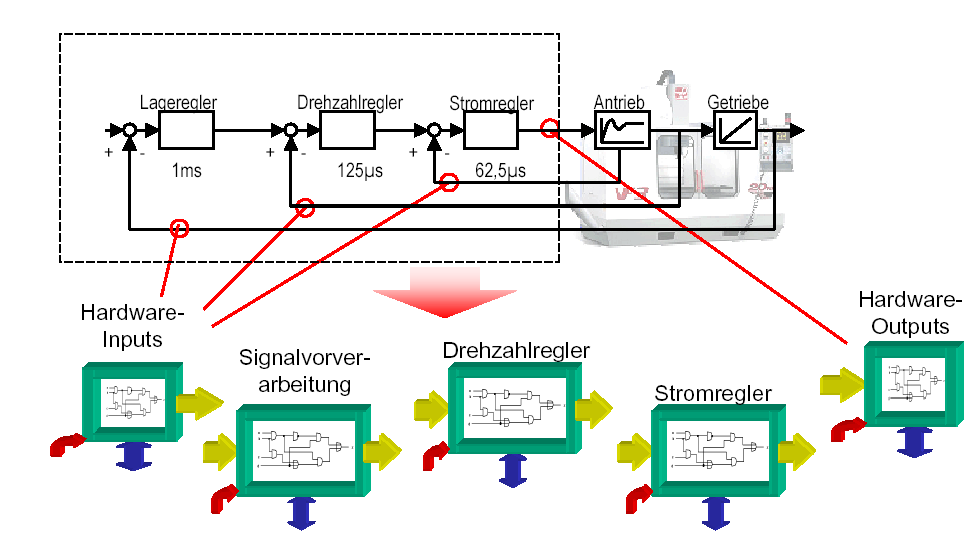
\includegraphics[width=15cm]{Beispielsprojekt}
\caption{Beispielsprojekt}\label{test}
\end{center}

\end{figure}
\newline
Standard Regelkreis: 
\begin{itemize}
	\item Lageregler: Eing�nge {\itshape xSoll[32], xIst[32]} und Ausgang {\itshape nSoll[32]}
	\item Drehzahlregler: Eing�nge {\itshape nSoll[32], nIst[32]} und Ausgang {\itshape iSoll[10]}
	\item Stromregler: Eing�nge {\itshape iSoll[10], iIst[10]} und Ausgang {\itshape stell[10]}
\end{itemize}

Zus�tzlich:
\begin{itemize}
	\item Signalvorverabeitung: Eing�nge {\itshape xIst-raw, nIst-raw, iIst-raw} und Ausg�nge {\itshape xIst[32], nIst[32], iIst[10]}
	\item HardwareInputs: Ausgang {\itshape xIst-raw, nIst-raw, iIst-raw}
	\item HardwareOutput: Eingang {\itshape stell[10]}
\end{itemize}
Die Zahlen in den eckigen Klammer geben die Bitbreite an.
\par

\section {Beispielprojekt  anlegen}
Bevor man mit dem Layout f�r den Antriebsregler anfangen kann, muss zun�chts einmal das Projekt angelegt werden. Dazu muss man folgenderma�en vorgehen:
\begin{enumerate}
	\item In der Men�leiste {\bf Project} den Eintrag {\bf New} ausw�hlen
	\item Im Dialog {\bf Select/Create project directory} den gew�nschten Pfad angeben
	\item Den Button {\bf Create New Directory} anklicken
	\item Name des Projekt eingeben und mit Return best�tigen
	\item Den neu erzeugten Ordner anw�hlen und den Button {\bf Open} dr�cken
	\item Die Datei {\bf project.xlm} anw�hlen und den Button {\bf Open} dr�cken
\end{enumerate}
Nach dem Anlegen und �ffnen des neuen Projekt wird das Arbeitsfenster mit einem leeren Layout ge�ffnet.
\section{Funktionsbl�cke erzeugen und konfigurieren}
Zur Realisierung des Antriebreglers ben�tigt man verschiedene Typen von Bl�cken und zwar:
\begin{itemize}
	\item 2 I/O-Bl�cke, einen f�r HardwareInput und einen fur HardwareOutput
	\item 3 CPU-Bl�cke f�r Signalverarbeitung, Drehzahlregler und Lageregler
	\item 1 Core-Block f�r Stromregler
\end{itemize}
\subsection{HardwareInput- und HardwareOutput-Block}
HardwareInput- und HardwareOutput-Block bilden die Schnittstelle nach Au�en. Daher werden I/O-Bl�cke verwendet. Die ankommenden Signale werden �ber den HardwareInput-Block an den Singalverarbeitungsblock weitergeleitet. Signale, die nach Au�en weitergeleitet werden m�ssen, kommen in den HardwareOutput-Block. Als erstes wird der HardwareInput erzeugt und konfiguriert:
\begin{enumerate} 
	\item Einen I/O-Block aus der Blockbiliothek per Drag'n Drop ziehen, d.h. mit dem Mauszeiger den Block ankilcken, die Maustaste dabei gedr�ckt lassen, den Block ins Arbeitsfenster ziehen und die Maustaste wieder loslassen.
	\item Im Dialog {\bf Block configuration} als erstes den Namen {\itshape "'HardwareInput"'} eingeben
	\item Unter {\bf Description} den Block beschreiben {\itshape "'...�ber diesen Inputblock werden die Signale weitergeleitet..."'}
	\item Den Offset Eintrag auf {\itshape "'Auto (0 ns)"'} lassen
	\item Unter {\bf Clock} den Takt f�r den Block angeben, d.h. {\itshape "'62,5 ns"'}
	\item Pins konfigurieren f�r die 4 Ausg�nge:
		\begin{itemize}
			\item Pinnamen angeben
			\item Bitbreite angeben
			\item Adresse angeben	
		\end{itemize}
\end{enumerate}
